\subsection{Complementary Benchmark Diagnostics}
\label{sec:benchmark_diagnostics}

The tables above provide compact summaries, but averaging can conceal interactions between a backbone and an optimizer. Figures~\ref{fig:heatmap_mccf1_mcc_test} and~\ref{fig:heatmap_accuracy_accuracy_test} therefore show the protocol-aligned locked-test endpoint for every backbone--optimizer cell. Each cell reports the mean and standard deviation across the three common seeds; color encodes the mean.

\begin{figure}[!htbp]\centering
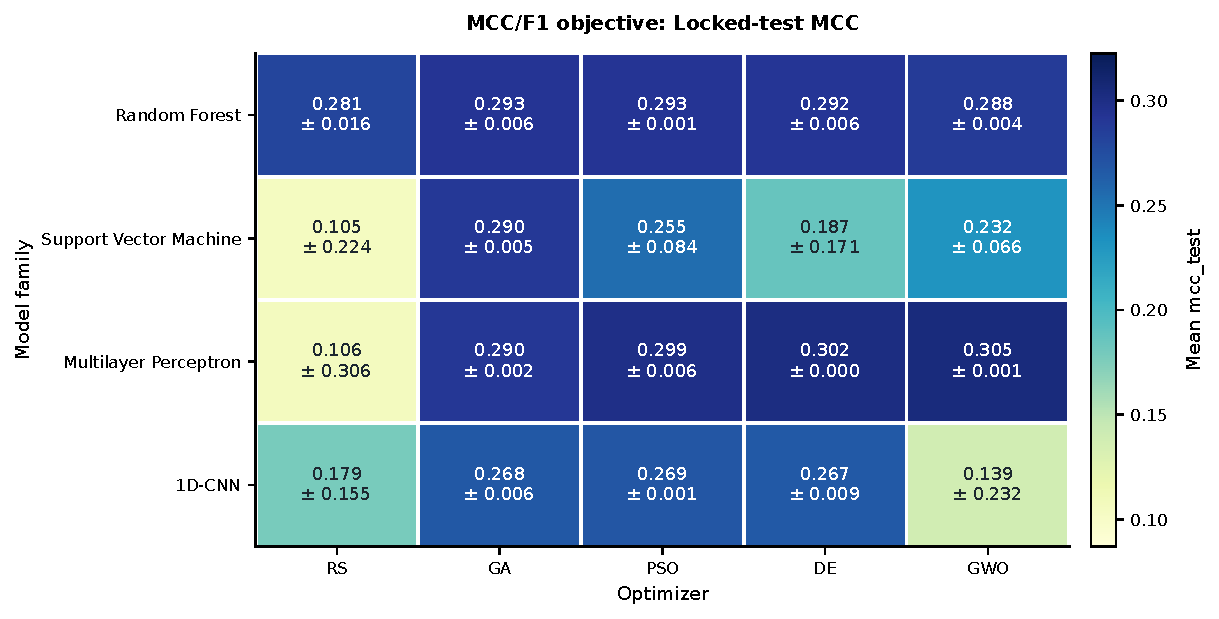
\includegraphics[width=0.95\linewidth]{figures/heatmap_mccf1_mcc_test.pdf}
\caption{Locked-test MCC by classifier backbone and optimizer after selection under MCC/$F_1$ fitness. Cells report the mean and standard deviation across the three common seeds; color encodes the mean.}
\label{fig:heatmap_mccf1_mcc_test}\end{figure}

\begin{figure}[!htbp]\centering
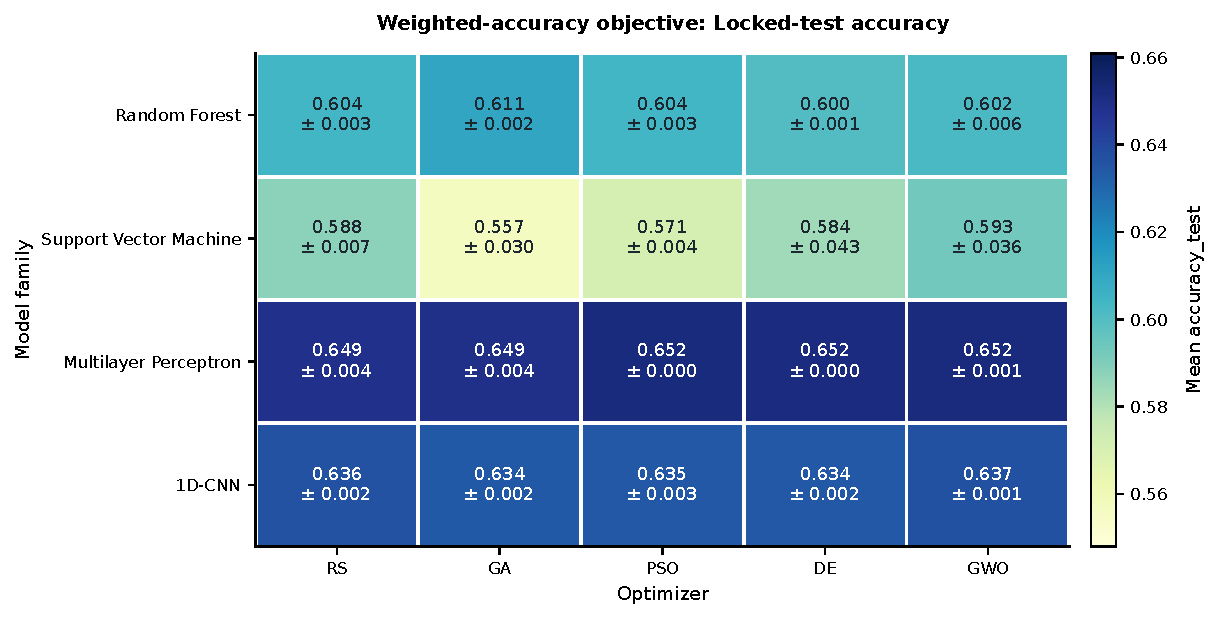
\includegraphics[width=0.95\linewidth]{figures/heatmap_accuracy_accuracy_test.pdf}
\caption{Locked-test accuracy by classifier backbone and optimizer after selection under weighted-accuracy fitness. Cells report the mean and standard deviation across the three common seeds; color encodes the mean.}
\label{fig:heatmap_accuracy_accuracy_test}\end{figure}

The heatmaps make the optimizer-by-backbone interaction visible at cell level. RF remains comparatively uniform across optimizers under MCC/$F_1$ fitness, whereas SVM, MLP, and 1D-CNN show greater variation. Under weighted-accuracy fitness, MLP forms the strongest row and 1D-CNN is competitive; SVM displays a wider optimizer-dependent range. These patterns are consistent with Table~\ref{tab:optimizer_primary_metrics}, while the small per-cell seed count means that color differences are descriptive rather than inferential.

Cell means can also obscure seed-level spread. Figure~\ref{fig:test_mcc_seed_distribution} displays all three locked-test MCC observations for each backbone--optimizer combination under both protocols, alongside the cell mean and standard deviation. Because each cell has only three observations, the raw values are more informative than a box-and-whisker summary.

\begin{figure}[!htbp]\centering
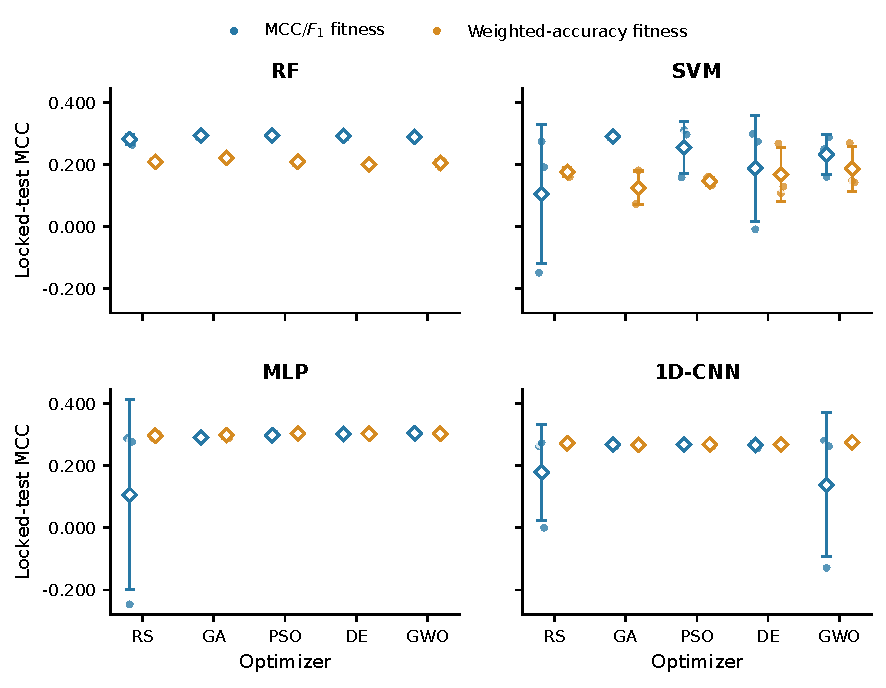
\includegraphics[width=0.95\linewidth]{figures/test_mcc_seed_points.pdf}
\caption{Locked-test MCC by optimizer and backbone under MCC/$F_1$ and weighted-accuracy fitness. Facets show the four backbones; points are the three common seed-level outcomes, and diamonds with vertical bars show the mean and one standard deviation. With three observations per cell, the display is descriptive rather than inferential.}
\label{fig:test_mcc_seed_distribution}\end{figure}

The raw points reveal a clear contrast in stability: RF outcomes remain tightly grouped, while several SVM and MLP cells show much wider seed-to-seed spread; 1D-CNN also has conspicuous dispersion for selected optimizers, including RS and GWO. Under weighted-accuracy fitness, the MLP and 1D-CNN MCC points are more tightly clustered, whereas some SVM cells remain dispersed. These patterns complement Table~\ref{tab:predictive_summary} and show how the protocol and backbone jointly shape run-to-run variation. With only three seeds per cell, however, the plot describes the observed runs and cannot establish the underlying variability distribution.

The Friedman analysis described above compares backbones within matched optimizer--seed blocks. A separate descriptive view addresses how optimizer ordering changes across backbones. Figure~\ref{fig:optimizer_average_ranks} reports average optimizer ranks across the 12 backbone--seed combinations within each protocol, using locked-test MCC or accuracy as appropriate.

\begin{figure}[!htbp]\centering
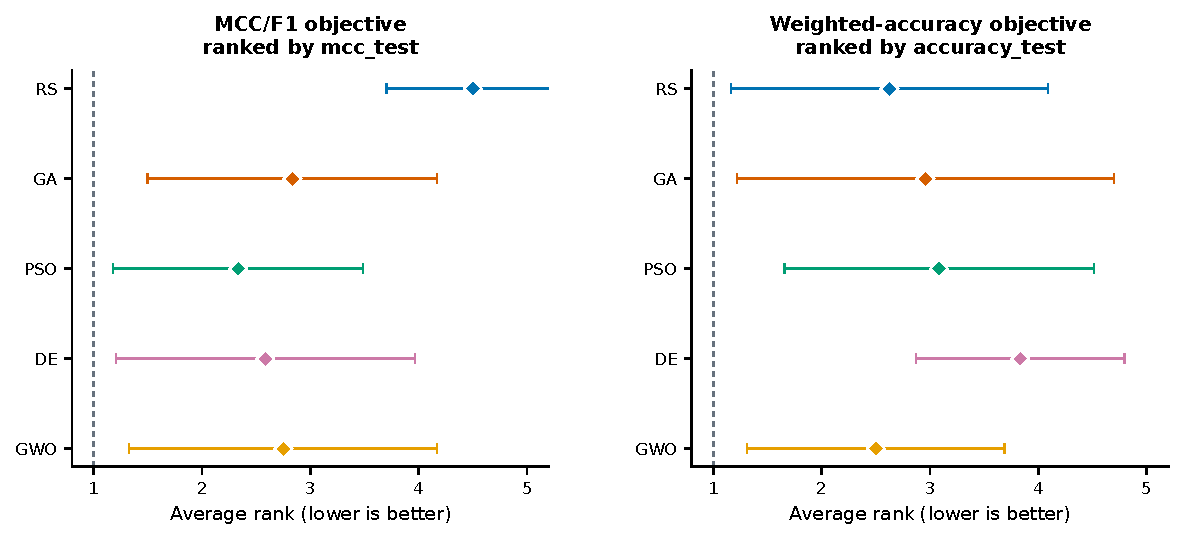
\includegraphics[width=0.95\linewidth]{figures/optimizer_average_ranks.pdf}
\caption{Descriptive average ranks of the five optimizers across 12 backbone--seed combinations (four backbones and three common seeds). Rankings use locked-test MCC under MCC/$F_1$ fitness and locked-test accuracy under weighted-accuracy fitness. Error bars show one standard deviation of block-level ranks; lower ranks indicate better ordering. This plot is descriptive and does not represent an optimizer significance test.}
\label{fig:optimizer_average_ranks}\end{figure}

The rank ordering changes between validation protocols and has substantial block-level spread, so no optimizer occupies a uniformly leading position across both endpoints. These ranks summarize ordering, not score magnitudes, and the 12 blocks share one chronological test interval; this plot therefore adds a descriptive view of heterogeneity rather than independent statistical evidence.

Finally, predictive score is only one consideration in a benchmark with non-negligible fitting effort. Figures~\ref{fig:performance_vs_fit_time_mccf1} and~\ref{fig:performance_vs_fit_time_accuracy} relate the protocol-aligned locked-test score to recorded candidate-fit time. Each panel represents one backbone; color and marker identify the optimizer, points give means over the three seeds, and vertical bars show one standard deviation in score. Within a panel, an upper-left position indicates a higher observed score at lower recorded fit time. Figure~\ref{fig:benchmark_radar} provides a normalized, multi-metric overview and is included only as a secondary summary because normalization removes the metrics' original units.

\begin{figure}[!htbp]\centering
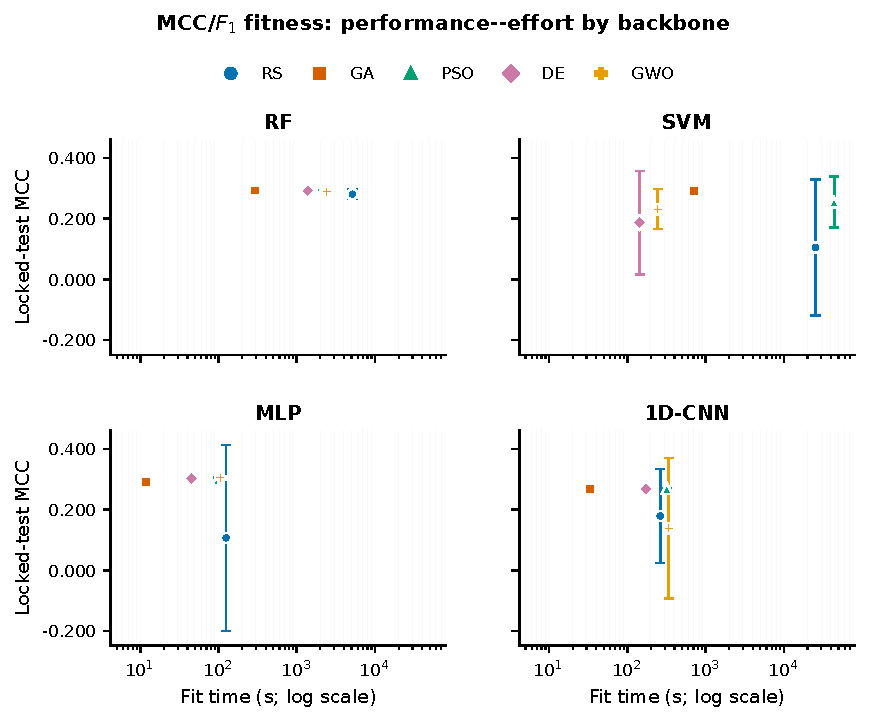
\includegraphics[width=0.95\linewidth]{figures/performance_vs_fit_time_mccf1.pdf}
\caption{Locked-test MCC versus mean cumulative uncached candidate-fit time under MCC/$F_1$ fitness. Separate panels show the four backbones; color and marker identify the optimizer. Points are means across three common seeds, with vertical bars indicating one standard deviation in test MCC. The horizontal axis is logarithmic and sums recorded fit times across candidates; it is not end-to-end optimizer wall-clock time.}
\label{fig:performance_vs_fit_time_mccf1}\end{figure}

\begin{figure}[!htbp]\centering
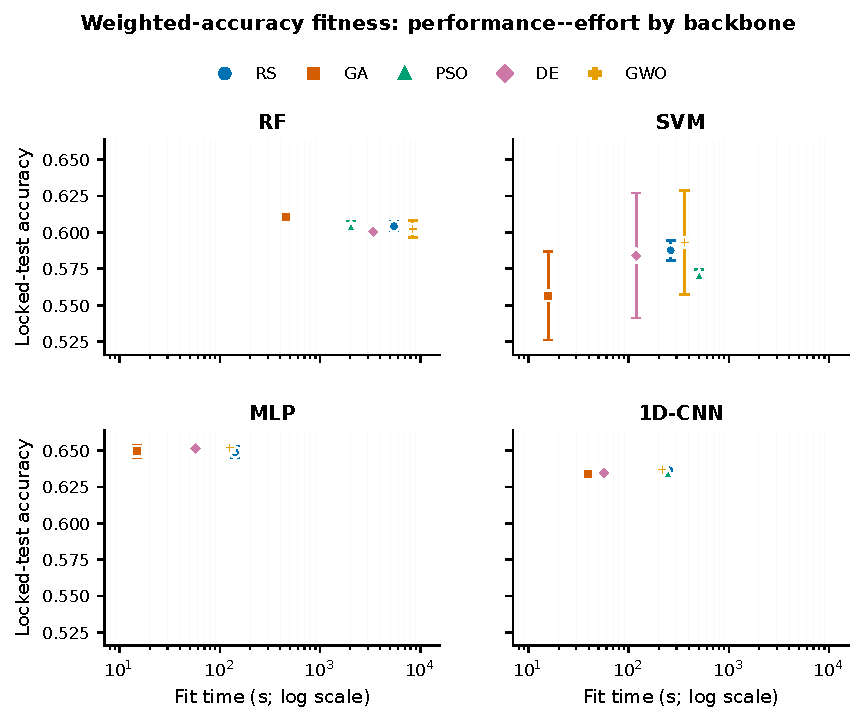
\includegraphics[width=0.95\linewidth]{figures/performance_vs_fit_time_accuracy.pdf}
\caption{Locked-test accuracy versus mean cumulative uncached candidate-fit time under weighted-accuracy fitness. Separate panels show the four backbones; color and marker identify the optimizer. Points are means across three common seeds, with vertical bars indicating one standard deviation in test accuracy. The horizontal axis is logarithmic and sums recorded fit times across candidates; it is not end-to-end optimizer wall-clock time.}
\label{fig:performance_vs_fit_time_accuracy}\end{figure}

\begin{figure}[!htbp]\centering
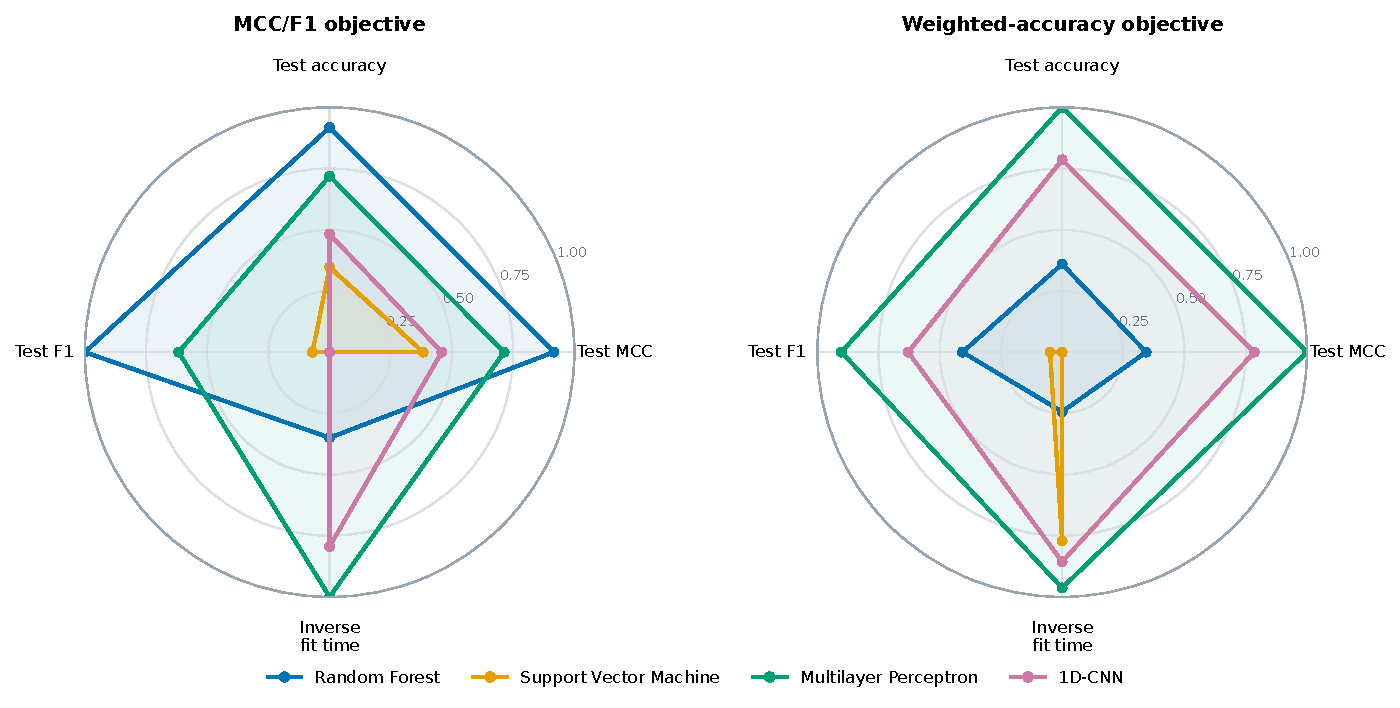
\includegraphics[width=0.95\linewidth]{figures/radar_overview_normalized.pdf}
\caption{Complementary normalized overview of locked-test MCC, accuracy, $F_1$, and inverse candidate-fit time by backbone and validation objective. Values are min--max normalized across the eight backbone--protocol averages; higher values indicate better values on each axis. Candidate-fit time is log-transformed before inversion and normalization.}
\label{fig:benchmark_radar}\end{figure}

The MCC/$F_1$ panels show that extra recorded fit time is not consistently accompanied by higher locked-test MCC: RF's optimizer means are tightly grouped despite differences in fit time, while SVM and MLP show optimizer-dependent score and seed-spread patterns. Under weighted-accuracy fitness, MLP and 1D-CNN occupy narrow accuracy ranges even where their fit-time positions differ; SVM shows a wider score range, but the more costly point is not uniformly the higher-scoring one. Thus, these observations do not support a general monotonic score--cost relationship. They describe cumulative uncached candidate fitting, not full search runtime, and should not be treated as an efficiency ranking. The radar profiles also vary by protocol and metric, reinforcing that no normalized shape can replace the original-scale results in Tables~\ref{tab:predictive_summary} and~\ref{tab:economic_summary}; it is a visual overview, not additional evidence for a ranking.
